% =====================================================================
%  main.tex — Relazione progetto Secure Cloud Computing (UNISA)
% =====================================================================
\documentclass[12pt,a4paper,oneside]{report}

% ---------------------------------------------------------------------
%  Lingua, codifica, font
% ---------------------------------------------------------------------
\usepackage[utf8]{inputenc}
\usepackage[T1]{fontenc}
\usepackage[english]{babel}
\usepackage{lmodern}
\usepackage{microtype}

% ---------------------------------------------------------------------
%  Layout pagina e interlinea
% ---------------------------------------------------------------------
\usepackage[a4paper,top=2.2cm,bottom=2.2cm,left=2.2cm,right=2.2cm]{geometry}

\usepackage{setspace}
\setstretch{1.2}

\setlength{\parindent}{0pt}
\setlength{\parskip}{0.4em}

% ---------------------------------------------------------------------
%  Colori
% ---------------------------------------------------------------------
\usepackage[table]{xcolor}

% Blu ardesia, desaturato
\definecolor{accent}{HTML}{3D5A80}
% Grigio-azzurro appena percettibile per le righe alternate
\definecolor{softgrey}{HTML}{F3F5F8}

% ---------------------------------------------------------------------
%  Titoli e sezioni
% ---------------------------------------------------------------------
\usepackage{titlesec}

\titleformat{\chapter}[hang]
    {\normalfont\LARGE\bfseries\color{black}}
    {\thechapter}{15pt}{}

\titlespacing*{\chapter}{0pt}{-15pt}{25pt}

\titleformat{\section}
    {\normalfont\Large\bfseries\color{black}}
    {\thesection}{0.8em}{}

\titlespacing*{\section}{0pt}{2em}{0.8em}

\titleformat{\subsection}
    {\normalfont\large\bfseries}
    {\thesubsection}{0.8em}{}

\titlespacing*{\subsection}{0pt}{1.5em}{0.6em}

\setcounter{secnumdepth}{3}
\setcounter{tocdepth}{2}

% ---------------------------------------------------------------------
%  Intestazioni e piè di pagina
% ---------------------------------------------------------------------
\usepackage{fancyhdr}

\pagestyle{fancy}
\fancyhf{}

\fancyhead[L]{\small Secure Cloud Computing}
\fancyhead[R]{\small Functional Architecture Document}

\fancyfoot[C]{\small\thepage}

\setlength{\headheight}{14pt}
\renewcommand{\headrulewidth}{0.3pt}
\renewcommand{\footrulewidth}{0pt}

\fancypagestyle{plain}{
    \fancyhf{}
    \fancyfoot[C]{\small\thepage}
    \renewcommand{\headrulewidth}{0pt}
}

% ---------------------------------------------------------------------
%  Tabelle
% ---------------------------------------------------------------------
\usepackage{array}
\usepackage{booktabs}
\usepackage{longtable}

\renewcommand{\arraystretch}{1.35}
\setlength{\tabcolsep}{6pt}

% Elimina le strisce bianche tra le regole booktabs e le righe colorate
\setlength{\aboverulesep}{0pt}
\setlength{\belowrulesep}{0pt}

% Linee booktabs dello stesso colore dell'intestazione:
%  - \toprule si fonde con l'intestazione colorata
%  - \midrule invisibile (l'intestazione separa già)
%  - \bottomrule chiude la tabella con una linea sottile
\setlength{\heavyrulewidth}{0.8pt}
\setlength{\lightrulewidth}{0pt}
\setlength{\cmidrulewidth}{0.4pt}
\arrayrulecolor{accent}

% Intestazione delle tabelle
\newcommand{\tablehead}[1]{%
    \textcolor{white}{\bfseries #1}%
}

% Riga dei requisiti
\newcommand{\reqrow}[3]{#1 & #2 & #3 \\}

% Titolo gruppo di requisiti
\newcommand{\reqgroup}[1]{%
    \par\vspace{0.8em}\noindent{\normalsize\bfseries #1}\par\nopagebreak\vspace{0.2em}%
}

% ---------------------------------------------------------------------
%  Figure e didascalie
% ---------------------------------------------------------------------
\usepackage{graphicx}
\usepackage{float}
\usepackage{caption}

\captionsetup{
    font=small,
    labelfont=bf
}

% ---------------------------------------------------------------------
%  Liste
% ---------------------------------------------------------------------
\usepackage{enumitem}
\setlist{itemsep=2pt}

% ---------------------------------------------------------------------
%  Utility
% ---------------------------------------------------------------------
\usepackage[hidelinks]{hyperref}
% =====================================================================
\begin{document}

% --- Parte iniziale (numerazione romana) ---
\pagenumbering{roman}

\hypersetup{pageanchor=false}
% =====================================================================
%  frontespizio.tex
% =====================================================================
\begin{titlepage}
\centering
\singlespacing

% --- Logo e ateneo ---------------------------------------------------

\includegraphics[width=0.28\linewidth]{attach/logo_standard.png}\par
\vspace{0.8cm}

{\LARGE\scshape Università degli Studi di Salerno\par}
\vspace{0.5cm}

{\large Department of Information and Electrical Engineering\\
and Applied Mathematics (DIEM)\par}
\vspace{0.3cm}
{\large Master's Degree in Computer Engineering\par}

\vfill

% --- Titolo ----------------------------------------------------------
{\color{accent}\rule{\linewidth}{0.8pt}}\par
\vspace{0.5cm}
{\Large\scshape Secure Cloud Computing\par}
\vspace{0.5cm}
{\fontsize{18}{24}\selectfont\bfseries
Cloud Architecture for Glucose Forecasting\\
in Type~1 Diabetes\par}
\vspace{0.4cm}
{\large\itshape Functional Architecture Document\par}
\vspace{0.5cm}
{\color{accent}\rule{\linewidth}{0.8pt}}\par

\vfill

% --- Docente e studenti ----------------------------------------------
\begin{minipage}[t]{0.38\linewidth}
\raggedright
\textbf{Professor}\\[0.15cm]
Prof. Angelo Marcelli
\end{minipage}%
\hfill
\begin{minipage}[t]{0.58\linewidth}
\raggedleft
\textbf{Students}\\[0.15cm]
\begin{tabular}{@{}l@{\hspace{1.2em}}r@{}}
Giovanni Lamberti    & IE22700272\\
Luigi Montonetti     & IE22700055\\
Vittorio Postiglione & IE22700189
\end{tabular}
\end{minipage}

\vspace{1.5cm}

% --- Anno accademico -------------------------------------------------
{\large Academic Year 2026/2027\par}

\end{titlepage}
\hypersetup{pageanchor=true}
% =====================================================================
%  abstract.tex
% =====================================================================
\chapter*{Abstract}
\addcontentsline{toc}{chapter}{Abstract}
\thispagestyle{plain}

% Colonna di testo più stretta e centrata (rientro di 1.8 cm per lato)
\begin{list}{}{%
    \setlength{\leftmargin}{1.5cm}%
    \setlength{\rightmargin}{1.5cm}%
    \setlength{\itemsep}{0pt}%
    \setlength{\parsep}{0.8em}%
    \setlength{\topsep}{0pt}}
\item[]
{\color{accent}\rule{\linewidth}{0.8pt}}

\vspace{0.6em}
This document describes the functional architecture of a
\emph{software-as-a-service} application that forecasts the glucose level of
patients with Type~1 diabetes thirty minutes after a meal.

Before eating, the patient declares the carbohydrates of the meal. A machine
learning model, fed with the patient's continuous glucose measurements,
predicts the glucose level, and the patient immediately receives one of four
outcomes: \emph{proceed}, \emph{proceed with a warning}, \emph{risk of
hyperglycemia} or \emph{risk of hypoglycemia}. Risky predictions are recorded
for the doctor, who reviews them periodically together with the trend of each
patient, while the center manager follows aggregated statistics on the use and
the performance of the service.

The document identifies the three actors and the data to acquire, and lists the
functional and non-functional requirements derived from the Service Level
Agreement: service from 6:00 to 22:00, availability and reliability of at least
99.5\%, response time within one second, 50\,000 customers and 5\,000 requests
per minute. It then describes eight use cases and illustrates the behavior of
the system through sequence diagrams. Implementation choices are deliberately
left to the following design phases.

\vspace{0.4em}
{\color{accent}\rule{\linewidth}{0.8pt}}

\vspace{0.2em}


\end{list}

% --- Corpo (numerazione araba) ---
\cleardoublepage
\pagenumbering{arabic}

% =====================================================================
%  capitoli/01_introduzione.tex
% =====================================================================
\chapter{Introduction}
\label{chap:introduzione}


\section{Purpose and scope}
This document defines \emph{what} the glucose monitoring system must do, not
\emph{how} it will be built. It describes the functional architecture of the service
chosen for Project~1 of the course: a machine learning model for time series
forecasting, delivered as a web application (SaaS) on a secure cloud
infrastructure. The document is written at a high level: it presents actors,
requirements, use cases, functional components and system behavior, and it
leaves out implementation details and technology stacks, which belong to later phases.

The system is used by three kinds of users: the patients, the doctors
(diabetologists) who follow them, and the manager of the center that runs the
service. Requirements are prioritized using the MoSCoW scheme: \emph{Must}
(M), \emph{Should} (S), \emph{Could} (C) and \emph{Won't} (W).

\section{How the system works}
At every meal the patient declares the amount of carbohydrates they intend to eat. A machine learning model, trained offline on historical patient cohorts, uses the patient's recent CGM measurements and the declared carbohydrates to estimate the glucose level thirty minutes later. 

The patient immediately receives one of four possible outcomes. Two of them
are risk outcomes, for which a flag is also recorded for the doctor. No instant
notification is sent: the doctor sees the flag at the next periodic review.

The doctor consults the history periodically, for example once a week, and
identifies the trends of each patient. 


The center manager observes the flow of
requests and the performance of the cloud service.

The application has two main purposes. For patients, it helps manage carbohydrate intake at each meal instead of relying on a fixed written diet. For doctors, it provides a way to monitor patients over time, compare predicted and measured glucose levels, and decide whether to contact the patient or adjust the diet.

The system does not suggest insulin doses and does not make therapeutic
decisions: the model only forecasts glucose at $+30$ minutes, and any decision
remains with the doctor.
\section{Actors}
The system has three actors. Each of them accesses only the data and the
functions related to their  role. 

\begin{table}[H]
\centering
\caption{Actors of the system.}
\label{tab:actors}
\small
\begin{tabular}{>{\bfseries\raggedright\arraybackslash}p{3.9cm}>{\raggedright\arraybackslash}p{6.8cm}>{\raggedright\arraybackslash}p{4.6cm}}
\toprule
\rowcolor{accent}\tablehead{Actor} & \tablehead{What the actor does} & \tablehead{What the actor sees}\\
\midrule
Patient & Enters the carbohydrates of every meal and receives the outcome of the prediction & Only his or her own data\\
\rowcolor{softgrey}
Doctor (diabetologist) & Registers new patients with their diet, monitors their glucose trend and records interventions & Only the patients in his or her care\\
Center manager & Monitors the overall operation of the service & Aggregated data only\\
\bottomrule
\end{tabular}
\end{table}

\section{Data acquisition}
Four streams of data enter the system:
\begin{itemize}
  \item \textbf{Carbohydrates and meal announcements.} Entered manually by the patient at each meal, indicating the amount of carbohydrates (in grams) planned for the meal as well as any snacks scheduled across the 30-minute horizon.
  \item \textbf{Continuous glucose monitoring (CGM).} Measured by a wearable sensor that records interstitial glucose every 5 minutes without manual intervention, providing an autoregressive sliding window of recent readings ($t-12 \dots t$). In this project, the physical sensor is simulated by replaying patient time series from the OhioT1DM dataset.
  \item \textbf{Insulin records.} Basal rates and bolus doses logged by the patient's continuous subcutaneous insulin infusion (CSII) pump or smart pen device, capturing physiological insulin-on-board.
  \item \textbf{Prescribed diet.} Established by the diabetologist for each patient, specifying target ranges and maximum carbohydrate thresholds for each meal.
\end{itemize}


% =====================================================================
\chapter{Requirements Analysis}
% =====================================================================

\vspace{0.5cm}

\section{Functional requirements}
The functional requirements, grouped by actor, describe what the system must
provide. The last column reports the Priority.

\begingroup
\small
\setlength{\LTpre}{4pt}\setlength{\LTpost}{6pt}

\reqgroup{Common functions}

\begin{longtable}{>{\bfseries}p{1.35cm}>{\raggedright\arraybackslash}p{\dimexpr\linewidth-2.95cm-6\tabcolsep\relax}>{\centering\arraybackslash}p{1.6cm}}
\toprule
\rowcolor{accent}\tablehead{ID} & \tablehead{Requirement} & \tablehead{Priority}\\
\midrule\endhead
\reqrow{RF01}{The system shall authenticate every user before any operation.}{M}
\rowcolor{softgrey}
\reqrow{RF02}{The system shall assign each account a role (patient, doctor, manager) and enable only the functions and the views of that role.}{M}
\bottomrule
\end{longtable}

\reqgroup{Patient}

\begin{longtable}{>{\bfseries}p{1.35cm}>{\raggedright\arraybackslash}p{\dimexpr\linewidth-2.95cm-6\tabcolsep\relax}>{\centering\arraybackslash}p{1.6cm}}
\toprule
\rowcolor{accent}\tablehead{ID} & \tablehead{Requirement} & \tablehead{Priority}\\
\midrule\endhead
\reqrow{RF03}{The patient shall declare the amount of carbohydrates (in grams) they intend to eat. The time of entry is recorded automatically.}{M}
\rowcolor{softgrey}
\reqrow{RF04}{The system shall automatically acquire the glucose level of the patient every 5 minutes through the CGM sensor (simulated via dataset replay).}{M}
\reqrow{RF05}{The system shall predict the patient's glucose level 30 minutes ahead, based on the recent CGM glucose history, meal carbohydrates and device inputs.}{M}
\rowcolor{softgrey}
\reqrow{RF06}{The system shall communicate to the patient one of the possible outcomes: \emph{regular}, the patient may proceed; \emph{carbohydrates above the diet} but glucose within the acceptable range, the patient may proceed but receives a warning; \emph{risk of hyperglycemia}; \emph{risk of hypoglycemia}.}{M}
\reqrow{RF07}{In case of predicted hyperglycemia or hypoglycemia, the system shall record a flag visible to the doctor in charge of the patient, without instant notification.}{M}
\rowcolor{softgrey}
\reqrow{RF08}{The patient shall be able to consult the history of their meals, glucose values and outcomes.}{C}
\bottomrule
\end{longtable}

\newpage

\reqgroup{Doctor}
\begin{longtable}{>{\bfseries}p{1.35cm}>{\raggedright\arraybackslash}p{\dimexpr\linewidth-2.95cm-6\tabcolsep\relax}>{\centering\arraybackslash}p{1.6cm}}
\toprule
\rowcolor{accent}\tablehead{ID} & \tablehead{Requirement} & \tablehead{Priority}\\
\midrule\endhead
\reqrow{RF09}{The doctor shall see in a table only the patients assigned to them, with the status of each patient and the flags received.}{M}
\rowcolor{softgrey}
\reqrow{RF10}{Once a patient is selected, the doctor shall see the trend over time: declared carbohydrates, measured glucose and 30-minute predictions.}{M}
\reqrow{RF11}{The system shall show the comparison between predicted and measured glucose and highlight the deviations.}{M}
\rowcolor{softgrey}
\reqrow{RF12}{The system shall indicate the trends, such as isolated episodes, frequent intake of carbohydrates above or below the diet, and recurring over- or underestimation errors of the model.}{S}
\reqrow{RF13}{The doctor shall be able to register a new patient and set their initial diet.}{M}
\rowcolor{softgrey}
\reqrow{RF14}{The doctor shall be able to update the prescribed diet of a patient.}{C}
\reqrow{RF15}{The doctor shall be able to record an intervention (reminder or diet change) and indicate its cause (model error or patient behavior).}{M}
\bottomrule
\end{longtable}

\reqgroup{Center manager}
\begin{longtable}{>{\bfseries}p{1.35cm}>{\raggedright\arraybackslash}p{\dimexpr\linewidth-2.95cm-6\tabcolsep\relax}>{\centering\arraybackslash}p{1.6cm}}
\toprule
\rowcolor{accent}\tablehead{ID} & \tablehead{Requirement} & \tablehead{Priority}\\
\midrule\endhead
\reqrow{RF16}{The manager shall have a dashboard with aggregated statistics, without access to the personal data of single patients.}{M}
\rowcolor{softgrey}
\reqrow{RF17}{The dashboard shall show the statistical interactions between doctors and patients.}{M}
\reqrow{RF18}{The dashboard shall show the performance of the service, such as response times, availability and compliance with the service level agreement.}{M}
\bottomrule
\end{longtable}

\reqgroup{Model and data}
\begin{longtable}{>{\bfseries}p{1.35cm}>{\raggedright\arraybackslash}p{\dimexpr\linewidth-2.95cm-6\tabcolsep\relax}>{\centering\arraybackslash}p{1.6cm}}
\toprule
\rowcolor{accent}\tablehead{ID} & \tablehead{Requirement} & \tablehead{Priority}\\
\midrule\endhead
\reqrow{RF19}{The system shall periodically update the prediction model, training it offline on the collected data, and make the new version available for predictions.}{M}
\rowcolor{softgrey}
\reqrow{RF20}{The system shall use a unified global model capable of serving all patients immediately (including newly registered patients), dynamically adapting to individual metabolic trends through the recent sliding-window time series without requiring per-patient retraining.}{M}
\reqrow{RF21}{The system shall detect how regularly each patient declares meals.}{C}
\bottomrule
\end{longtable}
\endgroup

\section{Non-functional requirements}
The ten non-functional requirements, grouped into four areas, derive from the
Service Level Agreement of the project and from the health nature of the data.

\begin{table}[H]
\centering
\caption{Performances that must be guaranteed according to the Service Level Agreement.}
\label{tab:sla}
\small
\begin{tabular}{p{4.6cm}p{9.3cm}}
\toprule
\rowcolor{accent}\tablehead{Target} & \tablehead{Value}\\
\midrule
Uptime & From 6:00 to 22:00, 7 days a week (16 hours per day) \\
\rowcolor{softgrey}
Availability & $\geq 99.5\%$ of the uptime (about 4.8 minutes of downtime per day) \\
Reliability & $\geq 99.5\%$ of the uptime \\
\rowcolor{softgrey}
Outage duration & At most 30 minutes, 3 minutes on average \\
Response time & $\leq 1$ second \\
\rowcolor{softgrey}
Customers & About 50\,000 \\
Prediction requests & Up to 5\,000 per minute \\
\rowcolor{softgrey}
Sensor samples & One every 5 minutes per patient \\
\bottomrule
\end{tabular}
\end{table}


\begingroup
\small
\setlength{\LTpre}{4pt}\setlength{\LTpost}{6pt}

\reqgroup{Performance and scalability}
\begin{longtable}{>{\bfseries}p{1.5cm}>{\raggedright\arraybackslash}p{\dimexpr\linewidth-3.1cm-6\tabcolsep\relax}>{\centering\arraybackslash}p{1.6cm}}
\toprule
\rowcolor{accent}\tablehead{ID} & \tablehead{Requirement} & \tablehead{Priority}\\
\midrule\endhead
\reqrow{RNF01}{The response time of a prediction, from the declared meal to the outcome, shall be $\leq 1$ s. If the value is not reachable during testing, additional resources or a revision of the service level agreement, agreed with the client, will be evaluated.}{M}
\rowcolor{softgrey}
\reqrow{RNF02}{The system shall sustain up to 5\,000 prediction requests per minute.}{M}
\reqrow{RNF03}{The system shall serve up to 50\,000 users in total.}{M}
\rowcolor{softgrey}
\reqrow{RNF04}{The system shall sustain the continuous acquisition of glucose samples, with one sample every 5 minutes for each monitored patient. The sizing considers the worst case in which almost all the 50\,000 expected users are patients, that is about 10\,000 writes per minute. It is assumed that glucose is acquired by a sensor with a 5-minute frequency.}{M}
\bottomrule
\end{longtable}

\reqgroup{Availability and reliability}
\begin{longtable}{>{\bfseries}p{1.5cm}>{\raggedright\arraybackslash}p{\dimexpr\linewidth-3.1cm-6\tabcolsep\relax}>{\centering\arraybackslash}p{1.6cm}}
\toprule
\rowcolor{accent}\tablehead{ID} & \tablehead{Requirement} & \tablehead{Priority}\\
\midrule\endhead
\reqrow{RNF05}{The service shall be active every day from 6:00 to 22:00, with availability and reliability $\geq 99.5\%$.}{M}
\rowcolor{softgrey}
\reqrow{RNF06}{Each outage shall last at most 30 minutes, with an average duration of 3 minutes.}{M}
\reqrow{RNF07}{Meals that are not declared or missing samples shall not cause errors: the system still produces an outcome, or reports it as not available.}{S}
\bottomrule
\end{longtable}

\reqgroup{Security and privacy}
\begin{longtable}{>{\bfseries}p{1.5cm}>{\raggedright\arraybackslash}p{\dimexpr\linewidth-3.1cm-6\tabcolsep\relax}>{\centering\arraybackslash}p{1.6cm}}
\toprule
\rowcolor{accent}\tablehead{ID} & \tablehead{Requirement} & \tablehead{Priority}\\
\midrule\endhead
\reqrow{RNF08}{Each user shall access only the data of their role, with a server-side control: a doctor does not read the data of patients who are not assigned, and the manager does not read personal data.}{M}
\rowcolor{softgrey}
\reqrow{RNF09}{The security measures are defined according to the health nature of the processed data. In particular, health data are protected in transit and at rest, and the center manager accesses only aggregated statistics, without the personal data of single patients.}{M}
\bottomrule
\end{longtable}

\reqgroup{Maintainability}
\begin{longtable}{>{\bfseries}p{1.5cm}>{\raggedright\arraybackslash}p{\dimexpr\linewidth-3.1cm-6\tabcolsep\relax}>{\centering\arraybackslash}p{1.6cm}}
\toprule
\rowcolor{accent}\tablehead{ID} & \tablehead{Requirement} & \tablehead{Priority}\\
\midrule\endhead
\reqrow{RNF10}{The model can be replaced or retrained without stopping the service.}{S}
\bottomrule
\end{longtable}
\endgroup

% =====================================================================
\section{Use cases}
% =====================================================================
The system offers eight use cases for the three actors, and all of them must include
UC01, as shown in the use case diagram. The prediction, the recording of the flag and the comparison with the
value measured by the sensor are internal steps of the system and are not
use cases.

\begin{table}[H]
\centering
\caption{Use cases and the requirements they cover.}
\label{tab:usecases}
\small
\begin{tabular}{>{\bfseries}p{1.2cm}p{5.9cm}p{2.3cm}p{4.5cm}}
\toprule
\rowcolor{accent}\tablehead{ID} & \tablehead{Use case} & \tablehead{Actor} & \tablehead{Requirements}\\

\midrule
UC01 & Log in & All & RF01, RF02, RNF08\\
\rowcolor{softgrey}
UC02 & Declare a meal and receive the outcome & Patient & RF03, RF04, RF05, RF06, RF07, RF20, RNF01\\
UC03 & View own history & Patient & RF08\\
\rowcolor{softgrey}
UC04 & View the list of patients & Doctor & RF09, RNF08\\
UC05 & Analyze the trend of a patient & Doctor & RF10, RF11, RF12, RF21\\
\rowcolor{softgrey}
UC06 & Record an intervention & Doctor & RF14, RF15\\
UC07 & Register a new patient & Doctor & RF13, RF20\\
\rowcolor{softgrey}
UC08 & View the service dashboard & Manager & RF16, RF17, RF18, RNF09\\
\bottomrule
\end{tabular}
\end{table}


\subsection{Use Case Diagram}

\begin{figure}[H]
\centering
    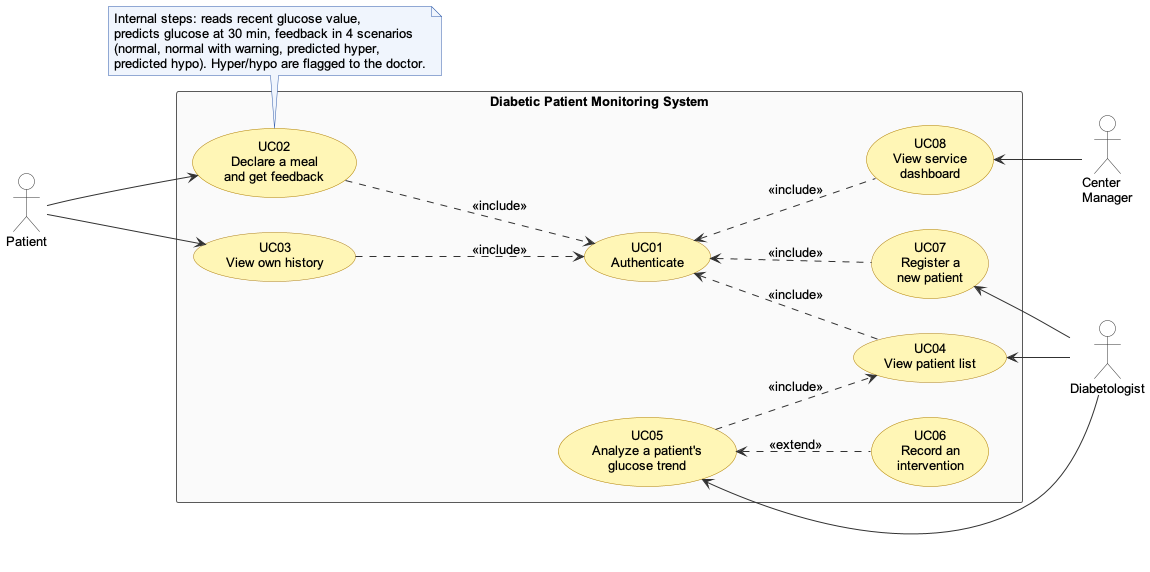
\includegraphics[width=1.0\linewidth]{attach/use_cases_v3.png}
    \caption{Use case diagram illustrating the interactions between patients, diabetologists, and center managers with the system's core functionalities.}
    \label{fig:placeholder}
\end{figure}
% =====================================================================
\chapter{Functional architecture}
% =====================================================================
The architecture is described in two parts. The \emph{online} part is the
service that handles requests from patients, doctors and the manager. The
\emph{offline} part concerns the training of the prediction model, which
supports the online service and is separate from the normal handling of
requests.

\section{Online architecture}
Figure~\ref{fig:architecture} shows the functional components of the online
service. The three actors reach the system through a single access control
component, which sends each request only to the service the role is entitled
to: the patient to their own data, the doctor to the assigned patients, and
the manager to aggregated data only. The services read and write a common data
archive. The CGM sensor writes the glucose samples directly into the archive,
in a flow that is separate from the prediction requests. The prediction service
uses the model made available by the offline training process.

\begin{figure}[H]
    \centering
    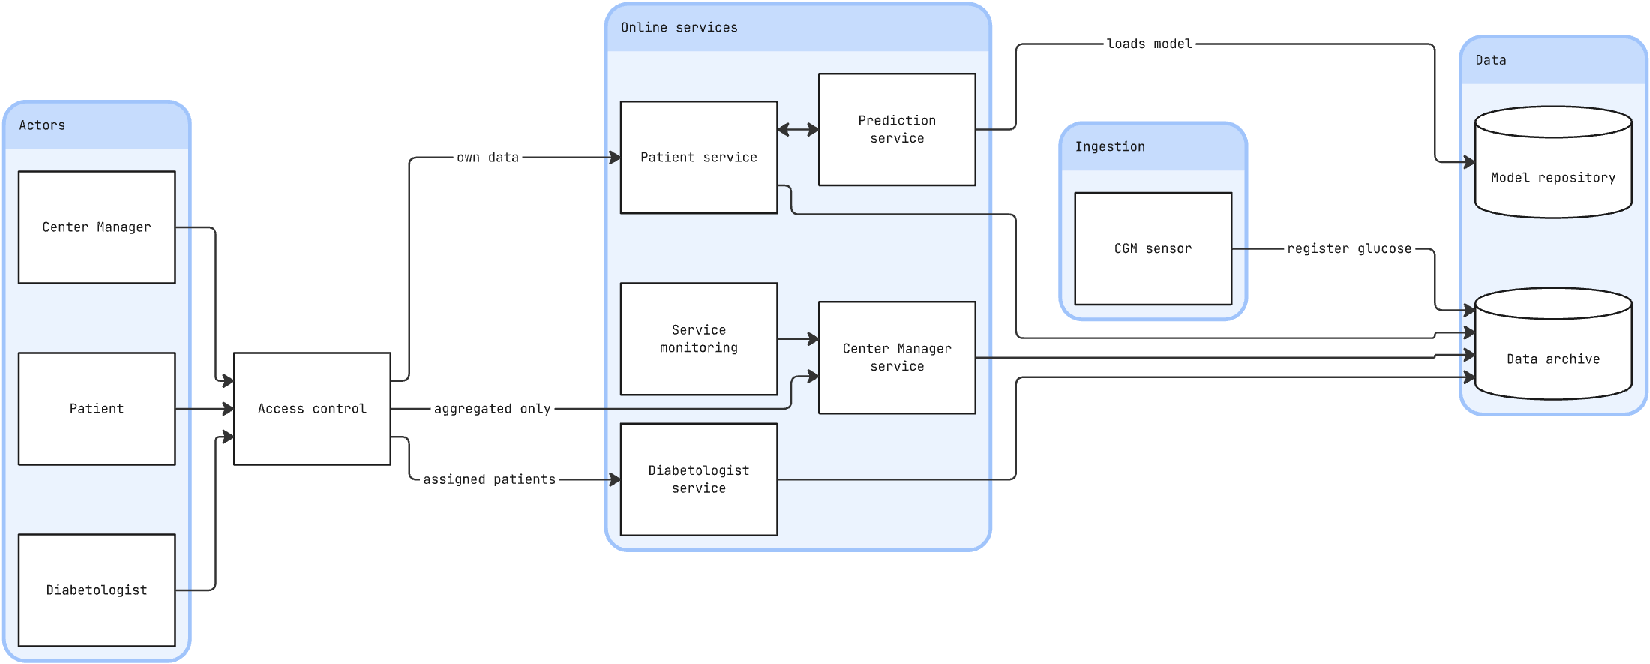
\includegraphics[width=1\linewidth]{attach/architecture.pdf}
    \caption{Functional architecture of the online service.}
    \label{fig:architecture}
\end{figure}


\section{Offline model training}
\label{sec:offline}
The system includes an offline process for training the prediction model
using historical patient data. The resulting model is made available to
the online service, which uses it to generate glucose predictions.
The training process is separate from the normal operation of the
online service and does not interfere with patient requests (RF19, RNF10).

The prediction engine relies on a unified global model trained on multicentric
patient cohorts (OhioT1DM dataset). Rather than maintaining thousands of isolated
per-patient models—which would introduce cold-start latency and severe memory overhead
in the cloud cluster—the model dynamically adapts to each individual's metabolic state
through their real-time autoregressive history (the preceding 60 minutes of glucose readings
and derivative trends). This design guarantees immediate availability for newly registered
patients while keeping cloud serving lightweight and horizontally scalable (RF20).

\section{Components}
Table~\ref{tab:components} describes each component of
Figure~\ref{fig:architecture}: what it does and which requirements it
satisfies.

\begingroup
\small
\setlength{\LTpre}{4pt}\setlength{\LTpost}{6pt}
\begin{longtable}{>{\bfseries\raggedright\arraybackslash}p{2.9cm}>{\raggedright\arraybackslash}p{\dimexpr\linewidth-5.6cm-6\tabcolsep\relax}>{\raggedright\arraybackslash}p{2.7cm}}\caption{Components of the online architecture, their responsibilities and requirements.}
\label{tab:components}\\
\toprule
\rowcolor{accent}\tablehead{Component} & \tablehead{What it does} & \tablehead{Requirements}\\
\midrule\endfirsthead
\toprule
\rowcolor{accent}\tablehead{Component} & \tablehead{What it does} & \tablehead{Requirements}\\
\midrule\endhead
\bottomrule\endfoot
Access control & Authenticates every user, assigns the role and forwards each request only to the service the role is entitled to. The control is made on the server and applies to the data, not only to the screens. & RF01, RF02, RNF08, RNF09\\
\rowcolor{softgrey}
Patient service & Receives the carbohydrates declared for a meal, reads the recent history of the patient, asks the prediction service for the 30-minute forecast, returns the outcome message, records a flag for the doctor when hyperglycemia or hypoglycemia is predicted, and gives the patient access to their own history. & RF03, RF05--RF08, RNF01, RNF07\\
Prediction service & Loads the unified prediction model from the model repository and computes the 30-minute glucose forecast and risk classification from recent CGM measurements and meal inputs. Serves all patients immediately without per-patient retraining. & RF05, RF20, RNF01, RNF02\\
\rowcolor{softgrey}
Diabetologist service & Shows the doctor the table of the assigned patients with their flags, the trend of each patient, the comparison between predicted and measured glucose with the deviations, and the detected trends. Allows registering new patients, setting and updating the diet, and recording interventions. & RF09--RF15, RF21, RNF08\\
Center Manager service & Builds the aggregated statistics shown in the dashboard, such as the interventions by cause, the accuracy of the predictions and the average regularity of the patients, without exposing the data of single patients. & RF16, RF17, RF18, RNF09\\
\rowcolor{softgrey}
Service monitoring & Collects response times, availability and compliance with the service level agreement, and passes them to the Center Manager service. & RF18, RNF01, RNF05, RNF06\\
CGM sensor & In this project it is simulated by replaying time series from the OhioT1DM dataset. Produces one glucose sample every five minutes for each monitored patient and registers it in the data archive. & RF04, RNF04\\
\rowcolor{softgrey}
Data archive & Stores meals and carbohydrates, measured glucose, predictions and deviations, flags, diets, assignments of patients to doctors and interventions. & RF03--RF18, RNF04\\
Model repository & Holds the validated versions and cryptographic checksums of the prediction model produced by offline training. New versions can be deployed via rolling updates without service interruption. & RF19, RNF10\\
\end{longtable}
\endgroup

\section{Access control}
Each actor accesses only the data and the functions of their competence.
The rule applies both to the data and to the views of the application. The check is made by the server (RNF08), and the health data are
protected in transit and at rest (RNF09).

\begin{figure}[H]
    \centering
    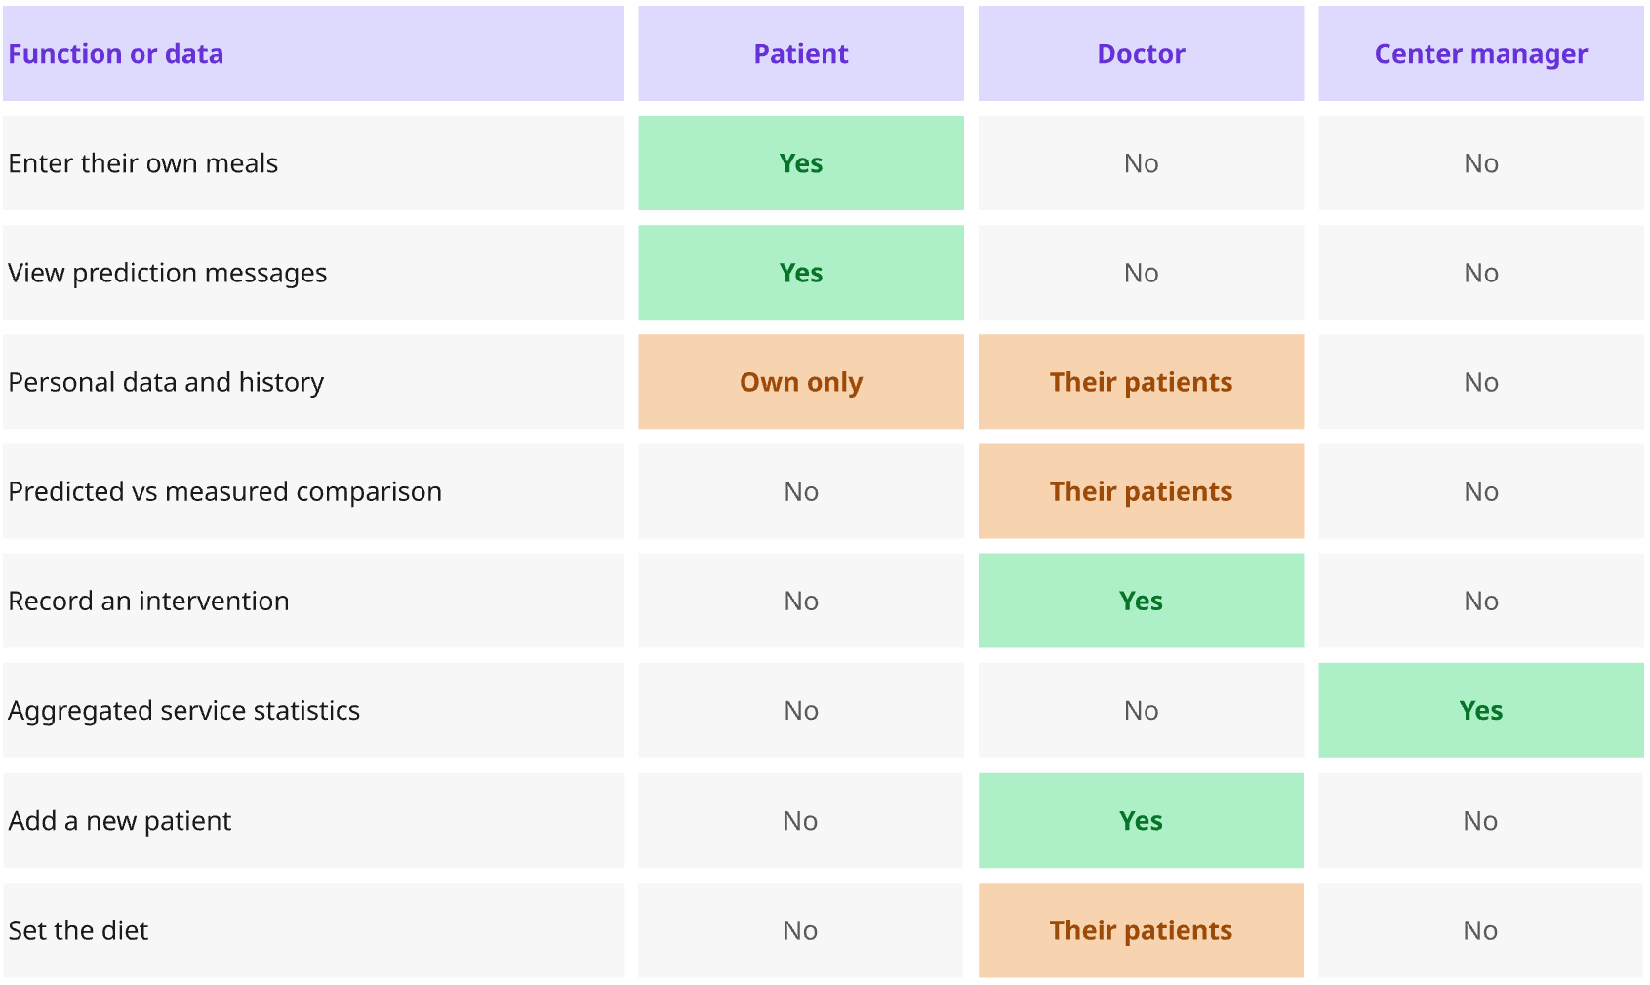
\includegraphics[width=\linewidth]{attach/permissions_table.pdf}
    \caption{Permissions of each actor.}
    \label{fig:permissions}
\end{figure}

% =====================================================================
\section{System behavior}
% =====================================================================
This section shows how the components interact in the main use cases through
sequence diagrams. In every diagram the access component first checks the
identity and the role of the user (UC01). 

\subsection{The patient declares a meal (UC02)}
Figure~\ref{fig:seq-meal} shows the core of the application. The patient logs
in and enters the carbohydrates of the meal. The patient service reads the
recent history of the patient from the data archive, passes a window of data
and the declared carbohydrates to the model, and receives the glucose predicted
at thirty minutes. The meal and the prediction are saved, and the outcome
depends on the prediction:
\begin{itemize}
  \item if the prediction is within the limits, the patient may proceed, with a
  warning if the carbohydrates exceed the diet;
  \item if hyperglycemia is predicted, the patient is told that the amount is
  excessive and a flag for the doctor is recorded;
  \item if hypoglycemia is predicted, the patient is told that the amount is
  insufficient and a flag for the doctor is recorded.
\end{itemize}
The doctor does not receive an instant notification and sees the flag during the
periodic review.

Under the hood, the prediction engine classifies the projected glucose into the seven clinical risk bands standard in diabetology (OhioT1DM benchmark). The system maps these granular clinical tiers into the four patient-facing macro-outcomes: target levels correspond to \emph{regular}; borderline levels trigger a \emph{warning}; and values below 3.9\,mmol/L (70\,mg/dL) or above 10.0\,mmol/L (180\,mg/dL) trigger the respective \emph{hypoglycemia} or \emph{hyperglycemia} risk flags.

\begin{figure}[H]
\centering
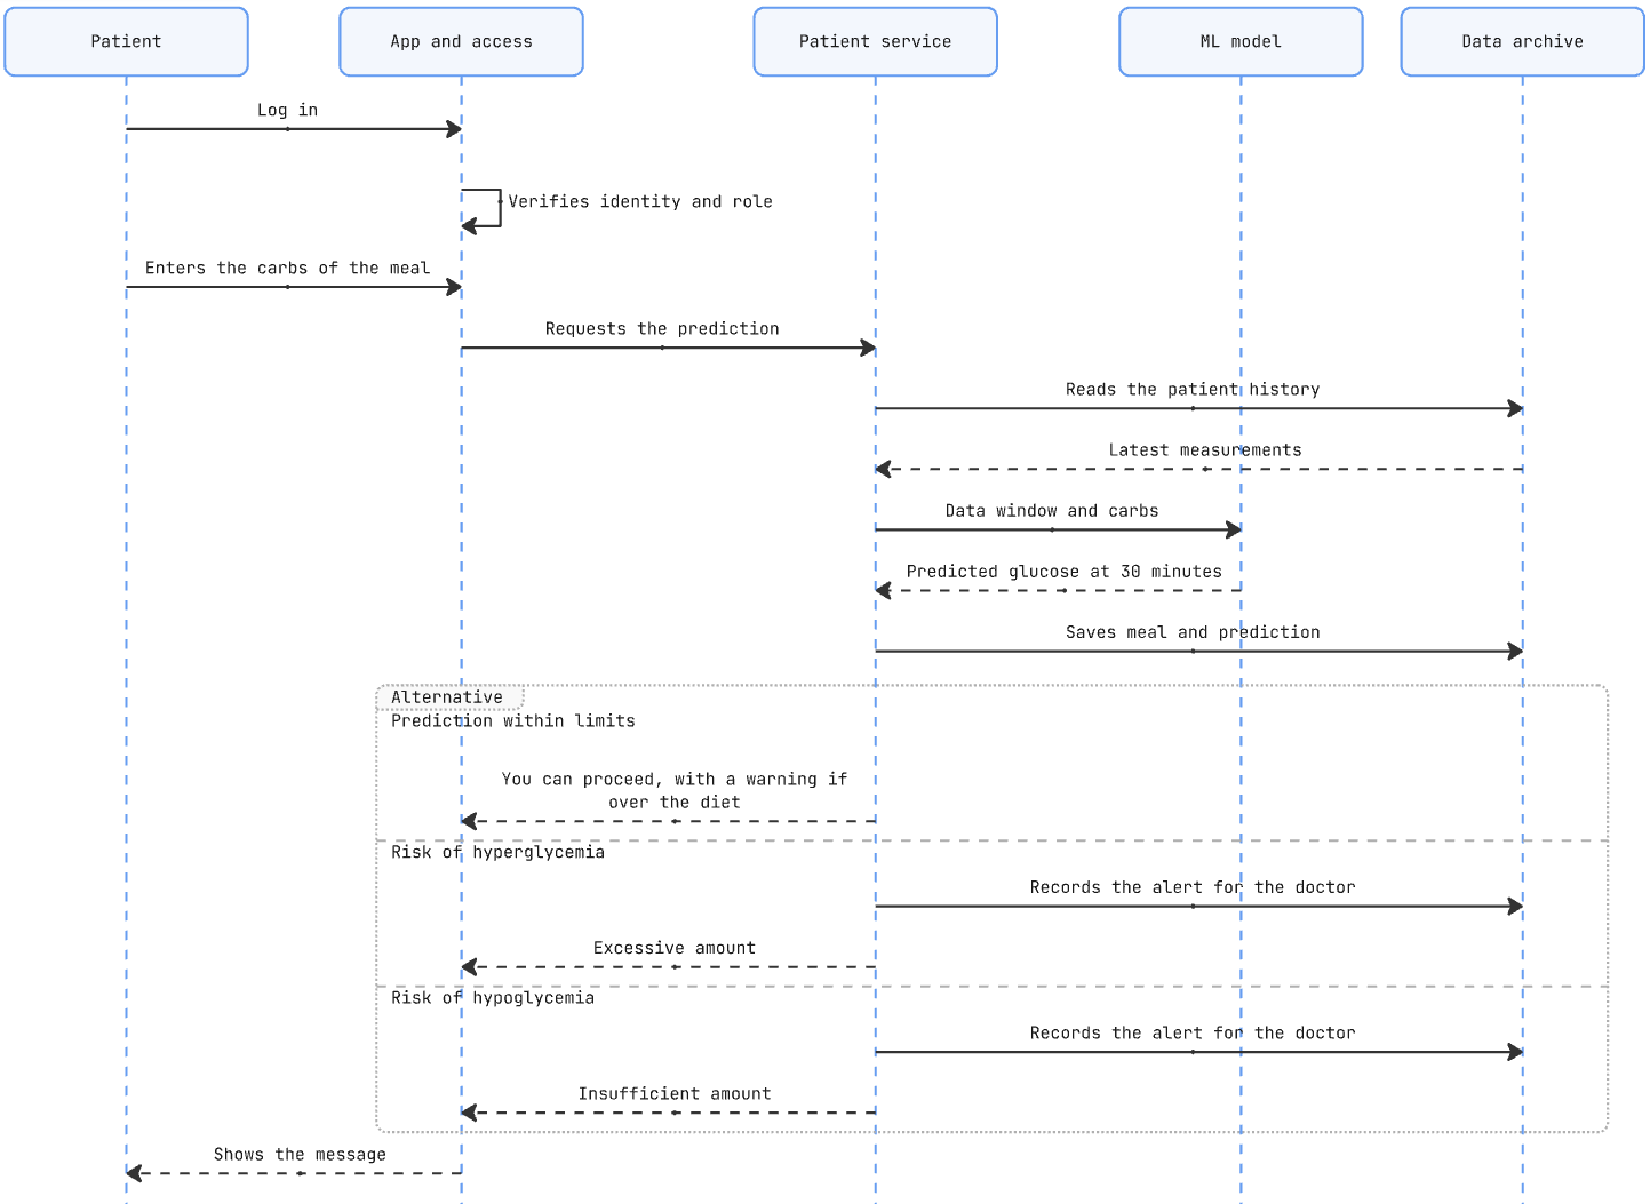
\includegraphics[width=\linewidth,height=0.76\textheight,keepaspectratio]{attach/seq_patient_meal.pdf}
\caption{Sequence diagram: the patient declares a meal and receives the outcome.}
\label{fig:seq-meal}
\end{figure}

\subsection{The doctor reviews the patients (UC04, UC05, UC06)}
In the periodic review (Figure~\ref{fig:seq-review}) the doctor opens a table
with only the patients assigned to them, with the flags received. After
selecting a patient, the doctor sees the trend over time, with the predicted
values compared with the measured ones. Before reading the data, the doctor
service checks that the patient is really assigned to that doctor. If an
intervention is needed, such as a reminder or a change of the diet, the doctor
records it and indicates whether the cause is a model error or the behavior of
the patient.

\begin{figure}[H]
\centering
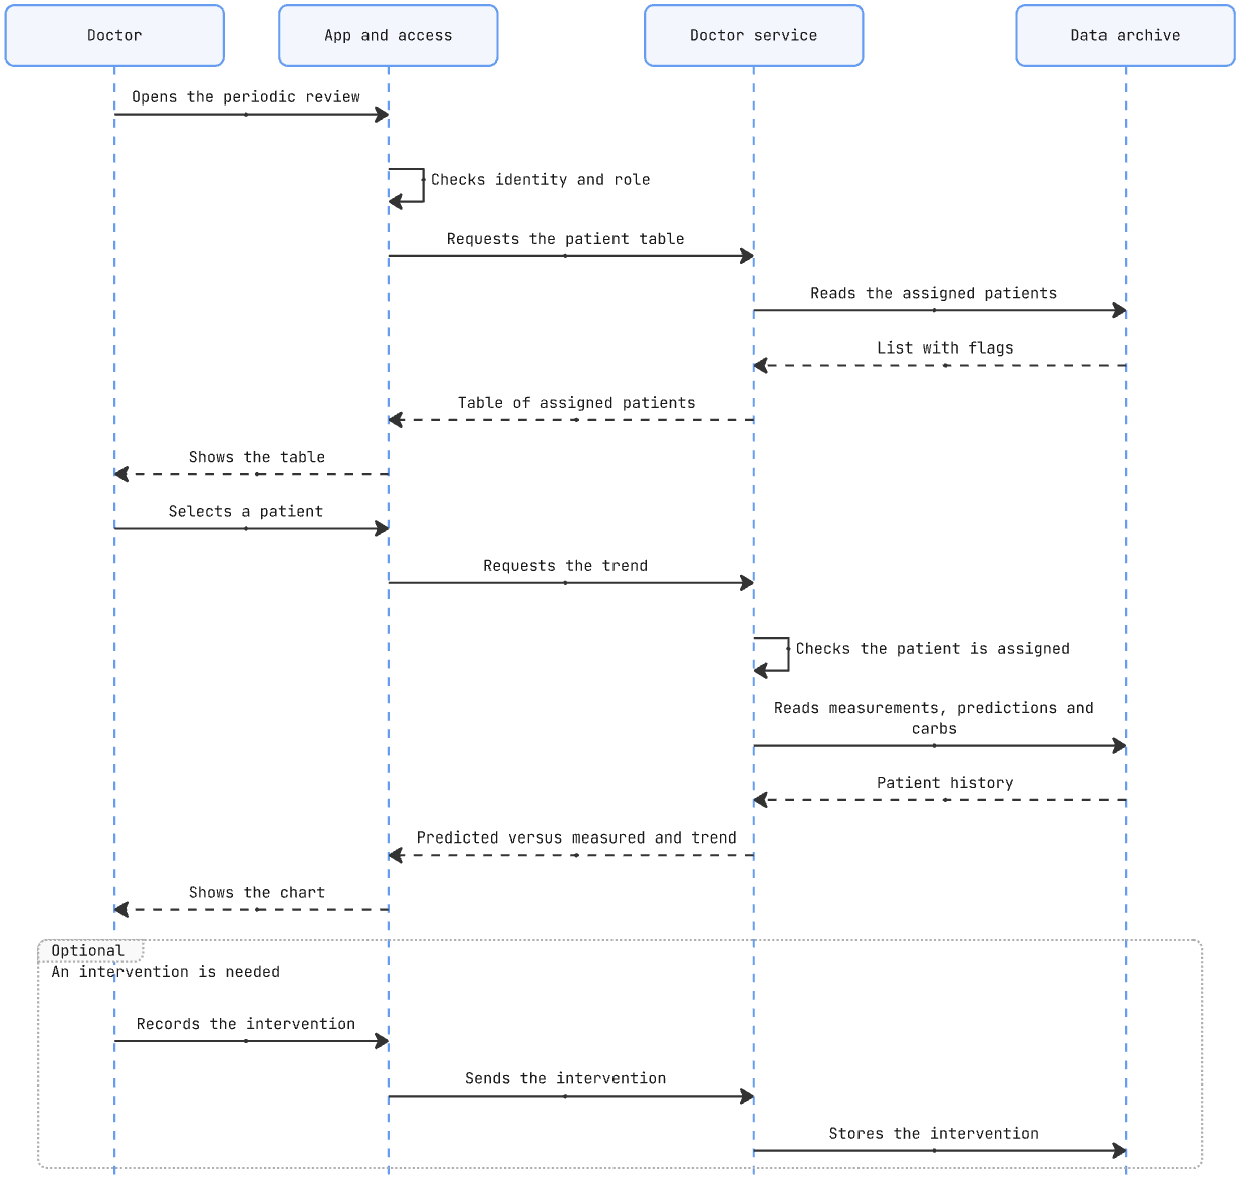
\includegraphics[width=\linewidth]{attach/seq_doctor_review.pdf}
\caption{Sequence diagram: the doctor reviews the assigned patients.}
\label{fig:seq-review}
\end{figure}

\subsection{The doctor registers a new patient (UC07)}
Figure~\ref{fig:seq-newpatient} shows how a new patient enters the system. The
doctor registers the patient, assigns them to their care, and sets the initial
diet. Thanks to the pre-trained unified global model, no per-patient retraining is
required; as soon as the initial 60-minute window of CGM readings is acquired,
the patient is immediately ready to receive predictions.

\begin{figure}[H]
\centering
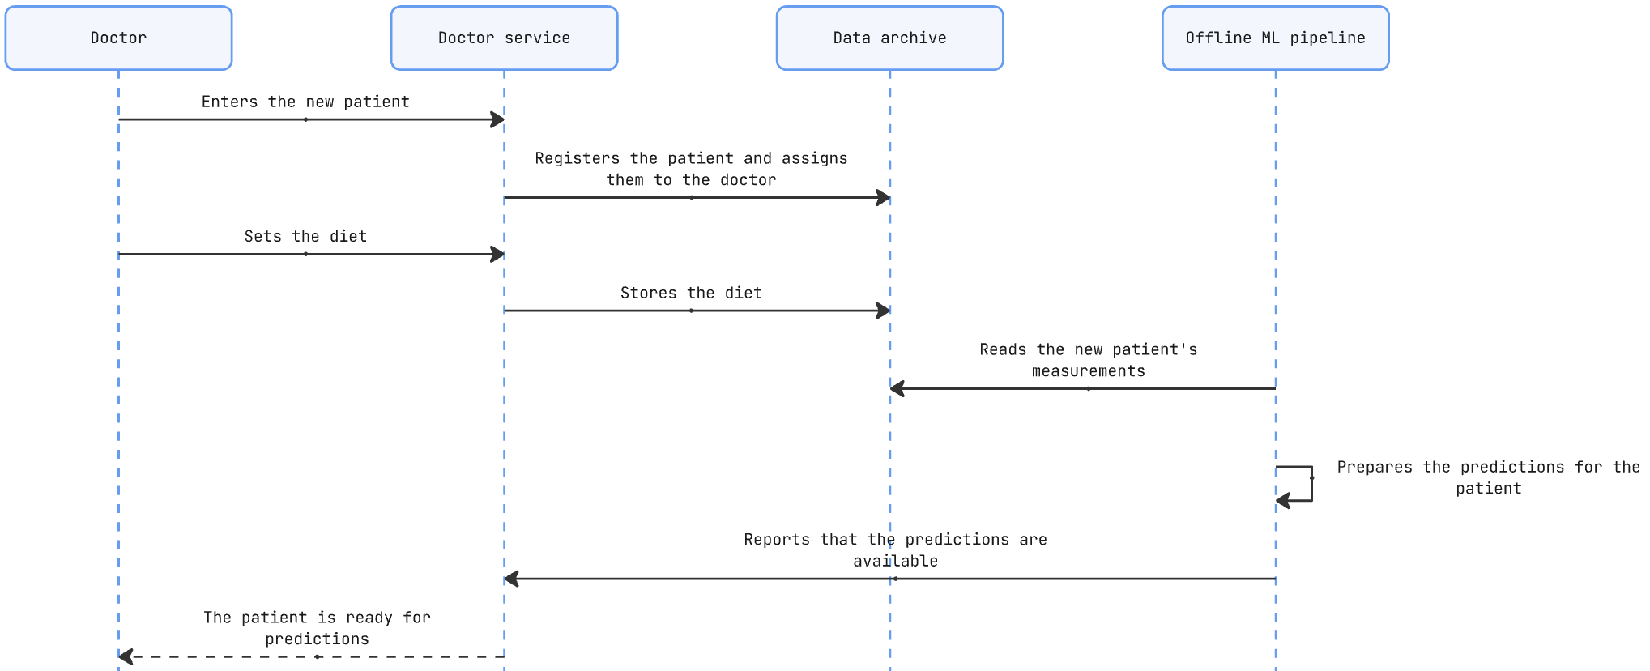
\includegraphics[width=\linewidth,height=0.72\textheight,keepaspectratio]{attach/seq_new_patient.pdf}
\caption{Sequence diagram: the doctor registers a new patient.}
\label{fig:seq-newpatient}
\end{figure}

\subsection{The center manager views the dashboard (UC08)}
The manager (Figure~\ref{fig:seq-dashboard}) opens the dashboard of the service
after logging in. The manager service reads counts and aggregated metrics from
the data archive: interventions by cause, accuracy of the predictions, average
regularity of the patients, response times and availability. It aggregates them
by period and by patient behavior, and returns aggregated statistics only. No
clinical data of single patients reaches the manager.

\begin{figure}[H]
\centering
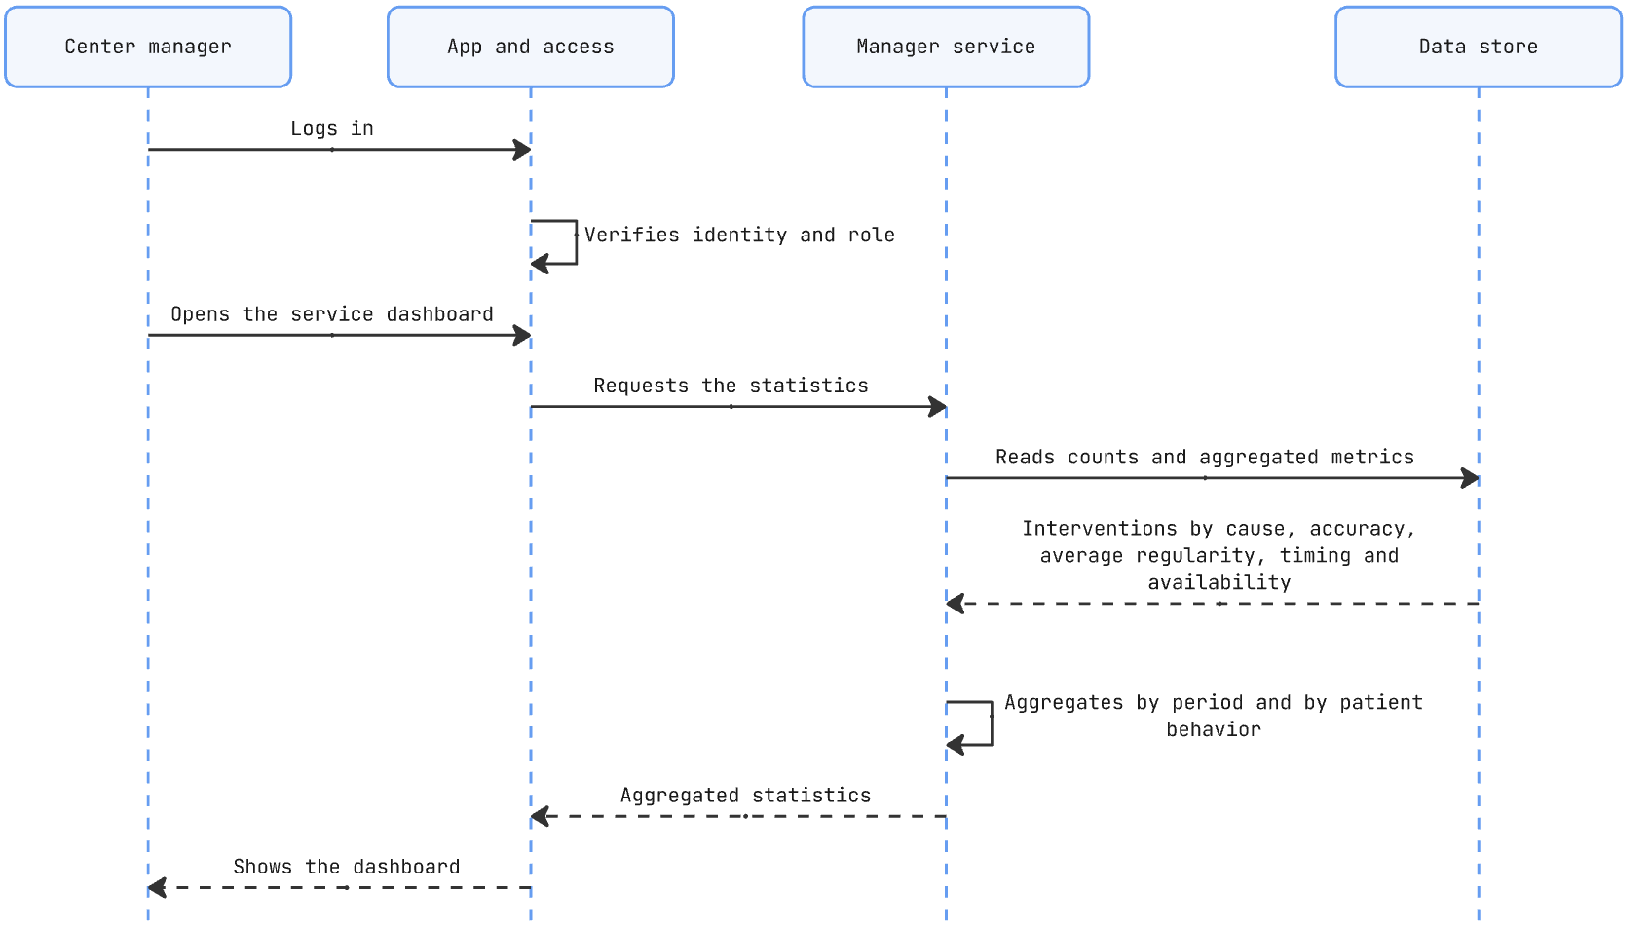
\includegraphics[width=\linewidth,height=0.72\textheight,keepaspectratio]{attach/seq_manager_dashboard.pdf}
\caption{Sequence diagram: the center manager views the service dashboard.}
\label{fig:seq-dashboard}
\end{figure}

\section{Mockups}
\label{sec:mockups}

To give an idea of what each actor sees, Figure~\ref{fig:mockups} shows
three early sketches of the main screens: the patient app, the doctor
dashboard and the center manager dashboard. They may differ in the final version of the application, which will have both mobile and desktop views.


\begin{figure}[htbp]
  \centering
  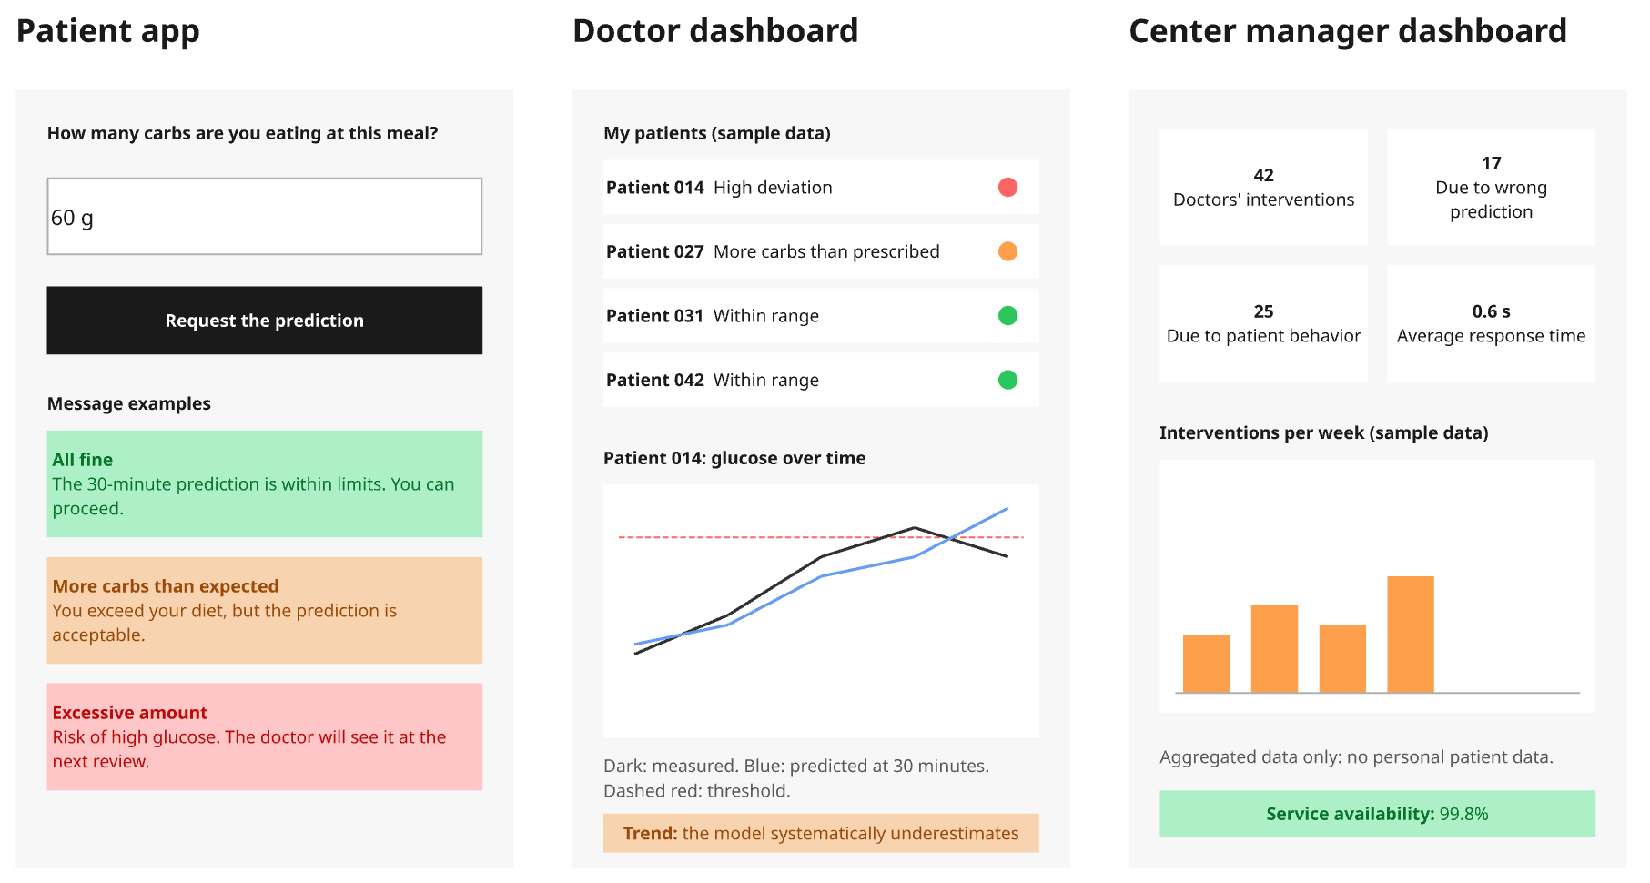
\includegraphics[width=\textwidth]{attach/mockup.pdf}
  \caption{Early mockups of the patient app, the doctor dashboard and the
  center manager dashboard (sample data).}
  \label{fig:mockups}
\end{figure}





\end{document}